% Options for packages loaded elsewhere
\PassOptionsToPackage{unicode}{hyperref}

% Set document class options
\documentclass[webpdf,large,contemporary,namedate]{oup-authoring-template}

% one column


%\usepackage{showframe}

% line numbers

% use upquote if available, for straight quotes in verbatim environments
\IfFileExists{upquote.sty}{\usepackage{upquote}}{}

% From Pandoc template for its feature
\usepackage{xcolor}
\usepackage{hyperref}

\hypersetup{
  pdftitle={Tolerance of hybrid hosts against infections, TAC Meeting December 2022},
  pdfkeywords={hybrids, parasites},
  breaklinks=true,
  bookmarks=true,
  hidelinks,
  pdfcreator={LaTeX via pandoc}}


% Pandoc syntax highlighting
\usepackage{color}
\usepackage{fancyvrb}
\newcommand{\VerbBar}{|}
\newcommand{\VERB}{\Verb[commandchars=\\\{\}]}
\DefineVerbatimEnvironment{Highlighting}{Verbatim}{commandchars=\\\{\}}
% Add ',fontsize=\small' for more characters per line
\usepackage{framed}
\definecolor{shadecolor}{RGB}{248,248,248}
\newenvironment{Shaded}{\begin{snugshade}}{\end{snugshade}}
\newcommand{\AlertTok}[1]{\textcolor[rgb]{0.94,0.16,0.16}{#1}}
\newcommand{\AnnotationTok}[1]{\textcolor[rgb]{0.56,0.35,0.01}{\textbf{\textit{#1}}}}
\newcommand{\AttributeTok}[1]{\textcolor[rgb]{0.77,0.63,0.00}{#1}}
\newcommand{\BaseNTok}[1]{\textcolor[rgb]{0.00,0.00,0.81}{#1}}
\newcommand{\BuiltInTok}[1]{#1}
\newcommand{\CharTok}[1]{\textcolor[rgb]{0.31,0.60,0.02}{#1}}
\newcommand{\CommentTok}[1]{\textcolor[rgb]{0.56,0.35,0.01}{\textit{#1}}}
\newcommand{\CommentVarTok}[1]{\textcolor[rgb]{0.56,0.35,0.01}{\textbf{\textit{#1}}}}
\newcommand{\ConstantTok}[1]{\textcolor[rgb]{0.00,0.00,0.00}{#1}}
\newcommand{\ControlFlowTok}[1]{\textcolor[rgb]{0.13,0.29,0.53}{\textbf{#1}}}
\newcommand{\DataTypeTok}[1]{\textcolor[rgb]{0.13,0.29,0.53}{#1}}
\newcommand{\DecValTok}[1]{\textcolor[rgb]{0.00,0.00,0.81}{#1}}
\newcommand{\DocumentationTok}[1]{\textcolor[rgb]{0.56,0.35,0.01}{\textbf{\textit{#1}}}}
\newcommand{\ErrorTok}[1]{\textcolor[rgb]{0.64,0.00,0.00}{\textbf{#1}}}
\newcommand{\ExtensionTok}[1]{#1}
\newcommand{\FloatTok}[1]{\textcolor[rgb]{0.00,0.00,0.81}{#1}}
\newcommand{\FunctionTok}[1]{\textcolor[rgb]{0.00,0.00,0.00}{#1}}
\newcommand{\ImportTok}[1]{#1}
\newcommand{\InformationTok}[1]{\textcolor[rgb]{0.56,0.35,0.01}{\textbf{\textit{#1}}}}
\newcommand{\KeywordTok}[1]{\textcolor[rgb]{0.13,0.29,0.53}{\textbf{#1}}}
\newcommand{\NormalTok}[1]{#1}
\newcommand{\OperatorTok}[1]{\textcolor[rgb]{0.81,0.36,0.00}{\textbf{#1}}}
\newcommand{\OtherTok}[1]{\textcolor[rgb]{0.56,0.35,0.01}{#1}}
\newcommand{\PreprocessorTok}[1]{\textcolor[rgb]{0.56,0.35,0.01}{\textit{#1}}}
\newcommand{\RegionMarkerTok}[1]{#1}
\newcommand{\SpecialCharTok}[1]{\textcolor[rgb]{0.00,0.00,0.00}{#1}}
\newcommand{\SpecialStringTok}[1]{\textcolor[rgb]{0.31,0.60,0.02}{#1}}
\newcommand{\StringTok}[1]{\textcolor[rgb]{0.31,0.60,0.02}{#1}}
\newcommand{\VariableTok}[1]{\textcolor[rgb]{0.00,0.00,0.00}{#1}}
\newcommand{\VerbatimStringTok}[1]{\textcolor[rgb]{0.31,0.60,0.02}{#1}}
\newcommand{\WarningTok}[1]{\textcolor[rgb]{0.56,0.35,0.01}{\textbf{\textit{#1}}}}

% tightlist command for lists without linebreak
\providecommand{\tightlist}{%
  \setlength{\itemsep}{0pt}\setlength{\parskip}{0pt}}




% Counters for addresses and footnotes
\newcounter{correspcnt} % For author footnotes
\renewcommand*{\thecorrespcnt}{\fnsymbol{correspcnt}}
\newcounter{addrcnt} % For author addresses

% Macros for dealing with affiliations, footnotes, etc.
\makeatletter

\def\MyNewLabel#1#2#3{\expandafter\gdef\csname #1@#2\endcsname{#3}}

\def\MyRef#1#2{\@ifundefined{#1@#2}{???}{\csname #1@#2\endcsname}}

\newcommand*\ifcounter[1]{%
  \ifcsname c@#1\endcsname
    \expandafter\@firstoftwo
  \else
    \expandafter\@secondoftwo
  \fi
}

\newcommand*\addrlblbycode[1]{%
  \ifcounter{ADDRLBL@#1}
    {}
    {\refstepcounter{addrcnt}\newcounter{ADDRLBL@#1}\setcounter{ADDRLBL@#1}{\value{addrcnt}}}%
    \arabic{ADDRLBL@#1}%
}

\newcommand*\addrbycode[1]{%
  \ifcounter{ADDR@#1}
    {}
    {\newcounter{ADDR@#1}%
     \address[\addrlblbycode{#1}]{\MyRef{ADDRTXT}{#1}}}%
}

\newcommand*\corresplblbycode[1]{%
  \ifcounter{CORRESPLBL@#1}
    {}
    {\refstepcounter{correspcnt}\newcounter{CORRESPLBL@#1}\setcounter{CORRESPLBL@#1}{\value{correspcnt}}}%
    \fnsymbol{CORRESPLBL@#1}%
}

\newcommand*\correspbycode[1]{%
  \ifcounter{CORRESP@#1}
    {}
    {\newcounter{CORRESP@#1}%
     \corresp[\corresplblbycode{#1}]{\MyRef{CORRESPTXT}{#1}}}%
}

\makeatother

% Add missing \city command mentioned in documentation but absent from cls
\providecommand\city[1]{#1}

% Create labels for Addresses if the are given in Elsevier format
   \MyNewLabel{ADDRTXT}{ABC}{%
  %
  \orgdiv{Department of Molecular Parasitology, Institute for
Biology}, %
  \orgname{Humboldt University Berlin (HU)}, %
  \orgaddress{%
   %
  \street{Philippstraße 13}, %
  %
  \city{Berlin}, %
  \state{10115}, %
  \country{Germany}%
  }%
   %
 %
 }
   \MyNewLabel{ADDRTXT}{DEF}{%
  %
  \orgdiv{Research Group Ecology and Evolution of Molecular
Parasite-Host Interactions}, %
  \orgname{Leibniz-Institut for Zoo and Wildlife Research (IZW)}, %
  \orgaddress{%
   %
  \street{Alfred-Kowalke-Straße 17}, %
  %
  \city{Berlin}, %
  \state{10315}, %
  \country{Germany}%
  }%
   %
 %
 }

% Create labels for Footnotes if they are given in Elsevier format
\MyNewLabel{CORRESPTXT}{1}{}
\MyNewLabel{CORRESPTXT}{2}{Current email address:
\href{mailto:fay.webster@hu-berlin.de}{fay.webster@hu-berlin.de)})}

% Pandoc header-include feature
\theoremstyle{thmstyleone}
\newtheorem{theorem}{Theorem}
\newtheorem{proposition}[theorem]{Proposition}
\theoremstyle{thmstyletwo}
\newtheorem{example}{Example}
\newtheorem{remark}{Remark}
\theoremstyle{thmstylethree}
\newtheorem{definition}{Definition}
% Pandoc header-include feature
\usepackage{booktabs}

\begin{document}

\journaltitle{Journal Title Here}
\DOI{DOI HERE}
\copyrightyear{YYYY}
\pubyear{YYYY}
\access{Advance Access Publication Date: Day Month Year}
\appnotes{Paper}

\firstpage{1}



\title[]{Tolerance of hybrid hosts against infections, TAC Meeting
December 2022}

\newcounter{thisauthcorresp} % For storage if author is corresponding author
\newcounter{thisauththanks} % For storage if author has thanks



\author[%
\addrlblbycode{ABC},\addrlblbycode{DEF}%
,\refstepcounter{correspcnt}\setcounter{thisauthcorresp}{\value{correspcnt}}\fnsymbol{thisauthcorresp}%
%
%
]{Fay Webster}

\addrbycode{ABC}
\addrbycode{DEF}

\corresp[\fnsymbol{thisauthcorresp}]{Corresponding author. \href{mailto:fay.webster@hu-berlin.de}{\nolinkurl{fay.webster@hu-berlin.de}}}




\author[%
\addrlblbycode{ABC},\addrlblbycode{DEF}%
%
%
,\corresplblbycode{2}%
]{Lubomír Bednář}

\addrbycode{ABC}
\addrbycode{DEF}




\correspbycode{2}


\author[%
\addrlblbycode{ABC},\addrlblbycode{DEF}%
%
%
,\corresplblbycode{1}%
]{Emanuel Heitlinger}

\addrbycode{ABC}
\addrbycode{DEF}




\correspbycode{1}


% Add author mark
\authormark{Fay Webster et al.}

\received{Date}{0}{Year}
\revised{Date}{0}{Year}
\accepted{Date}{0}{Year}

%\editor{Associate Editor: Name}

\abstract{
Parasites in hybrid zones can give insight into species barriers, as
they are modulating the fitness of hybrid hosts. Recent findings have
demonstrated lower infection intensities with parasites in hybrids in
the European House Mouse Hybrid zone (HMHZ), indicating higher disease
resistance. However, tolerance has not yet been addressed in depth, as
it is impractical to measure in wild populations. In an attempt to
predict and evaluate the health impact of parasite infections and
extrapolate tolerance in the HMHZ, we use a machine learning method. A
random forest model was trained on immune parameters measured in
experimental lab infections with Eimeria and then applied to data
obtained from field sampling. Our predictions revealed that these
infections are more detrimental to hybrid male mice. This approach
represents an initial step in assessing tolerance in field studies.}

\keywords{hybrids; parasites}


\maketitle


\hypertarget{introduction}{%
\section{Introduction}\label{introduction}}

\hypertarget{introduce-the-topic}{%
\subsection{Introduce the topic}\label{introduce-the-topic}}

\hypertarget{methods}{%
\section{Methods}\label{methods}}

\hypertarget{laboratory-infection-experiments}{%
\subsection{Laboratory infection
experiments}\label{laboratory-infection-experiments}}

\hypertarget{mouse-strains-luke}{%
\subsubsection{Mouse strains (Luke)}\label{mouse-strains-luke}}

In order to gain a better understanding of tolerance in hybrid mice we
established a laboratory model of experimental lab infections with the
Eimeria spp. Our experimental setup is a variation of the framework in
Balard et al., 2020. The mice used are four wild-derived inbred mouse
strains and their generated F1 hybrids. The mouse strains are fully
inbred, as they have pased through at least 20 generations of sibling
pairing. From the fours strains, two were used as a representation of
the M. m. domesticus: SCHUNT (Locality: Schweben, Hessen, Germany {[}N:
5°0 26', E: 9°36'{]} \citet{martincova2019phenotypic}) and STRA
(Locality: Straas, Bavaria, Germany {[}N: 50°11', E: 11°46'{]}
(\citet{pialek2008development}). The two following strains were in turn
derived from M. m. musculus: BUSNA (Locality: Buškovice, Bohemia, Czech
Republic {[}N: 5°0 14', E: 1°3 22'{]} (pialek2008development)) and PWD
(Locality: Kunratice, Bohemia, Czech Republic {[}N: 5°0 01', E: 14
2°9'{]} (\citet{gregorova2000pwd}). In our setup there are two two
intersubspecific hybrids (STRAxBUSNA and SCHUNTxPWD) and two
intrasubspecific hybrids (SCHUNTxSTRA and PWDxBUSNA). The mice were
between 5.6 and 21.4 weeks. The mice were acquired from the Institute of
Vertebrate Biology of the Czech Academy of Sciences in Studenec (license
number 61974/2017-MZE-17214; for further details on strains see
https://housemice.cz/en).

Infections with the parasite Eimeria induce a protective immune reaction
in the host against reinfection (Rose et al., 1992a; Smith \& Hayday,
2000). The feces of the naive mice were tested to ensure that the mice
were Eimeria spp., prior to infection, following the methods of Balard
\citet{balard2020coupling}.

\hypertarget{infections-with-eimeria-spp.-luke}{%
\subsubsection{Infections with Eimeria spp.
(Luke)}\label{infections-with-eimeria-spp.-luke}}

The procedure used is as described in in Balard et al., 2020. During the
infections mice were housed solo in cages. We infected the mice orally
with 150 sporulated oocysts of one Eimeria isolate suspended in 100 µl
phosphate-buffered saline (PBS). The mice had access to food and water
ad libitum SNIFF, Rat/Mouse maintenance feed 10 mm and were observed
daily for 8 days until their sacrifice by cervical dislocation. In the
case that individual mice showed severe adverse health effects or
extreme weigh loss of more than 18\% relative to their weight at the
start of experiment, were then sacrificed earlier at defined humane end
points (experiment license Reg. 0431/17). Daily measurements of weight
were recorded and fecal matter was gathered. Collected feces were
supspended in 2\% potassium dichromate and paaracite oocysts were
retrieved by NaCl flotation.

To enable a consistent distribution between experimental groups, mice
were allocated at random, while ensuring a similar distribution of age
and sex between groups.

\hypertarget{gene-expression-high-thoughput-qpcr-luke}{%
\subsubsection{Gene expression high-thoughput qPCR
(Luke)}\label{gene-expression-high-thoughput-qpcr-luke}}

Homogenized caecum tissue was processed for RNA using the filter based
innuPREP RNA Mini Kit 2.0 (Jena analytik, Germany) according to
manufacturer instructions. Extracted RNA was quantified using NanoDrop
2000c (Thermo Scientific, Waltham, USA) and transcribed into cDNA with
iScript (Bio-rad Laboratories, Hercules, California, United States),
following manufacturer protocol. Gene expression was ascertained via
hight-throughput qPCR of cDNA from the caecum extracted material, plated
onto Fluidigm IFC (integrated fluidic circuit), initialized by the Juno
controller and read in the Fluidigm BioMark HD (PN 100-7222 C1,
Fluidigm, South San Francisco, California, United States). After cDNA
conversion mentioned above, the samples went through the recommended
preparation steps, carried out in sterile extractor hood, with reagents
being kept at 4 °C when in use, and at -20 °C when stored overnight. All
pipetting was done using sterile filter tips. Table of wet-lab tested
primers can be found in the appendix file 20614FDGP21T1\_DESIGN

\hypertarget{specific-target-amplification-sta-using-fluidigm-preamp-master-mix-luke}{%
\subsubsection{Specific target amplification (STA) using Fluidigm PreAmp
master mix
(Luke)}\label{specific-target-amplification-sta-using-fluidigm-preamp-master-mix-luke}}

ll primers at 100µM were pooled together in a micro centrifuge tube and
resulting solution was diluted to a final concentration of 500 nM, with
a 10 mM Tris-HCl (pH 8,0), 0.1 mM EDTA TE Buffer (12090-015, Invitrogen,
Waltham, Massachusetts, United States). Fluidigm Preamp Master Mix
(Fluidigm PN 100-5580) was added to the solution according to the
manufacturer instructions, to create delta gene assay Preamp Master Mix.
Sample cDNA (including a non-template control (NTC)) was plated onto
96-well plates and the master mix added to each well. Sample plate was
then gently vortexed for 5 seconds and spun down at 1,000 x g for 1
minute. The amplification reactions were carried out in the Biometra
TOne 96 (846-2-070-301, Analytic Jena, Jena, Germany) at the following
cycling conditions: Hold at 95 ºC for 2 minutes, 95 ºC for 15 seconds,
then 60 ºC for 4 minutes (15x), Hold at 4 ºC for infinity.

\hypertarget{primers-and-sample-preparation-luke}{%
\subsubsection{Primers and sample preparation:
(Luke)}\label{primers-and-sample-preparation-luke}}

1.5 µL of primer (wet lab tested) at 100 µM ,13.5 µL of TE Buffer and 15
µL of 2X Assay Loading Reagent (PN 100-7611, Fluidigm), were combined to
create 10X Assay solutions. Sample reaction mixes were then created by
combining 1.8 µL of preamplified and Exonuclease I treated cDNA, 2 µL of
2X SsoFast EvaGreen Supermix with low ROX™ (Bio-Rad, PN 172-5211) and
192.24 Delta Gene Sample Reagent (PN 100-6653, Fluidigm), to create 4 µL
stock per 1 sample reaction. This was scaled to accommodate sample
repeat runs. Prepared samples and primers were stored at -20ºC until the
IFC chips were primed.

\hypertarget{ifc-qpcr-runs-luke}{%
\subsubsection{IFC qPCR runs (Luke)}\label{ifc-qpcr-runs-luke}}

The 192.24 IFC was plated and treated as per manufacturer instructions
(PN 100-7222 C1), consisting of control line fluid injection into
accumulator 2 slot, removal of protective film, pipetting of samples and
10X assay mixes in 3 µL volumes, adding 150 µL of Actuation Fluid (PN
100-6250) into the P1 port, 150 µL of Pressure Fluid (PN 100-6249) into
the P2 and P3 ports, 20 µL of Pressure Fluid into the P4 and P5 ports
and finally initializing the IFC in the Juno controller, using the Load
Mix 192.24 GE script. After the initialization completed, the IFC was
transferred into the BioMark HD and the assay properties were set as
follows: Application type: Gene Expression, Passive reference: ROX,
Assay: Single probe, Probe type: EvaGreen, using the GE 192x24 PCR+Melt
v2.pcl protocol, on Auto-exposure.

\hypertarget{wild-mice}{%
\subsection{Wild mice}\label{wild-mice}}

During the years 2016 to 2019, we sampled 1889 mice in the House Mouse
Hybrid zone. We used live traps to capture mice in farms and houses,
during September every year. To catch mice of \emph{M. musculus
musculus}, \emph{M. musculus domesticus} and hybrid origin, we selected
a large geographic area in Brandenburg and Neuruppin. For each mouse, we
have collected information during dissections, on their body length,
their weight and their pathophysiology. Tissue samples were used to
genotype the hosts. Further information on the set-up of the experiment
can be found in previous publications of the group
\citet{balard2020intensity} From 1889 mice, 336 were selected with a
varying genotype for Fluidigm BioMark assay. Another 95 were selected
for fluorescence-activated cell sorting.

\hypertarget{statistical-analysis}{%
\subsection{Statistical Analysis}\label{statistical-analysis}}

\hypertarget{imputation-of-missing-data}{%
\subsubsection{Imputation of missing
data}\label{imputation-of-missing-data}}

To make the most of our data collection, we aimed to resolve
missingness. Missing data were imputed using multiple imputations by
chained equations. We used the package MICE in R \citet{van2011mice},
with five imputed data sets and five iterations. Data generated by FACS
or the Gene Expression / Biomarker assay were regarded as missing if
each mouse had measurements for some variables. For each continuous
variable, we specified a predictive mean matching model. All the
remaining variables were used as predictors in the imputation. To
control the quality of our imputations, we evaluated the distribution
plot of the existing data and the imputed data for all measurements
\ref{fig:fig1} \ref{fig:fig2}. Further, we tested for convergence. We
assume data is ``missing completely at random'' or ``missing at
random''. For both types of missingness, multiple imputation is a
suggested method to impute missing variables \citet{van2018flexible}.

\hypertarget{questions-to-dos}{%
\paragraph{Questions / To-dos:}\label{questions-to-dos}}

\begin{enumerate}
\def\labelenumi{\arabic{enumi}.}
\tightlist
\item
  Should I log-transform the data prior to imputation?
\item
  Increasing produced data sets / iterations
\item
  sensitivity analyses using complete cases only
\end{enumerate}

\hypertarget{random-forest}{%
\subsubsection{Random forest}\label{random-forest}}

In an attempt to predict the health impact of infections in mice, we
used a random forest model \citet{breiman2001random}. We chose the
maximum weight loss during the experimental laboratory infections of
mice with the parasite \emph{Eimeria spp.} as a response variable.
Maximum weight loss is here used as a proxy describing the health impact
caused by infections. The random forest was constructed utilizing the
expression data of 20 genes, obtained by the biomarker assay (utilizing
the R package ``randomForest,'' ntree = 1000). The data set was split
into a training data set of 70 \% and to a testing data set of 30 \% to
avoid over-fitting and to assess the performance of the model on
``unseen'' data. As a quality assessment, we used k- fold cross
validation, where the data set is divided into k subsets. Each time, the
model is assessed by using one of the k subsets as the test data set and
the other as the training data set. The model was then fitted on each
k-subset and afterwards evaluated on the test set. Last the evaluation
score was noted and the model then discarded.

\begin{figure*}[th]
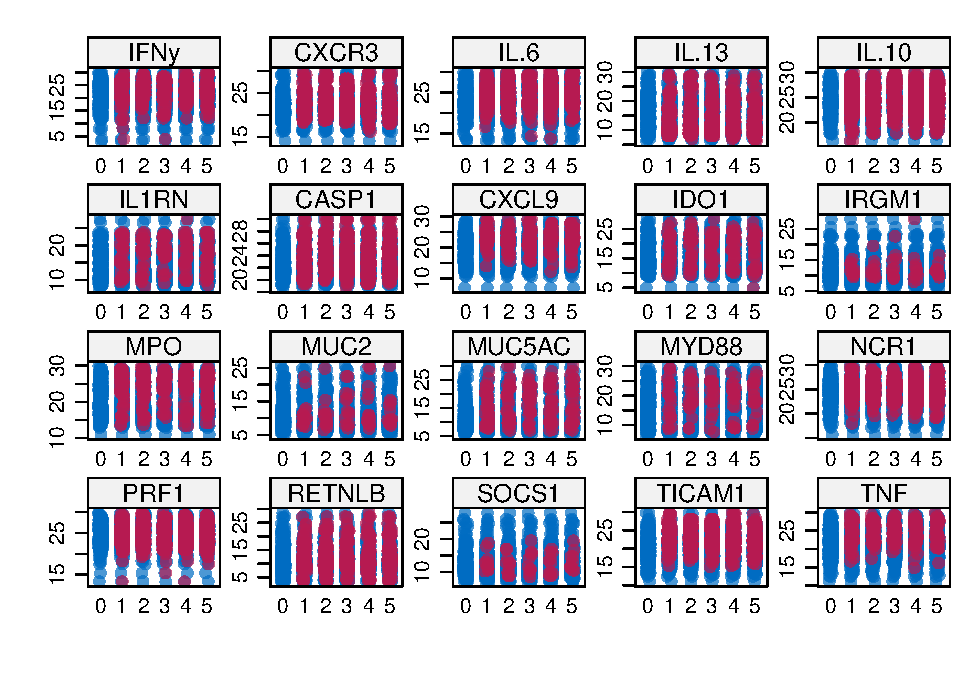
\includegraphics[width=1\linewidth]{Article_hybrids_tolerance_files/figure-latex/fig1-1} \caption{Stripplot of observed and imputed data}\label{fig:fig1}
\end{figure*}

\begin{figure*}[th]
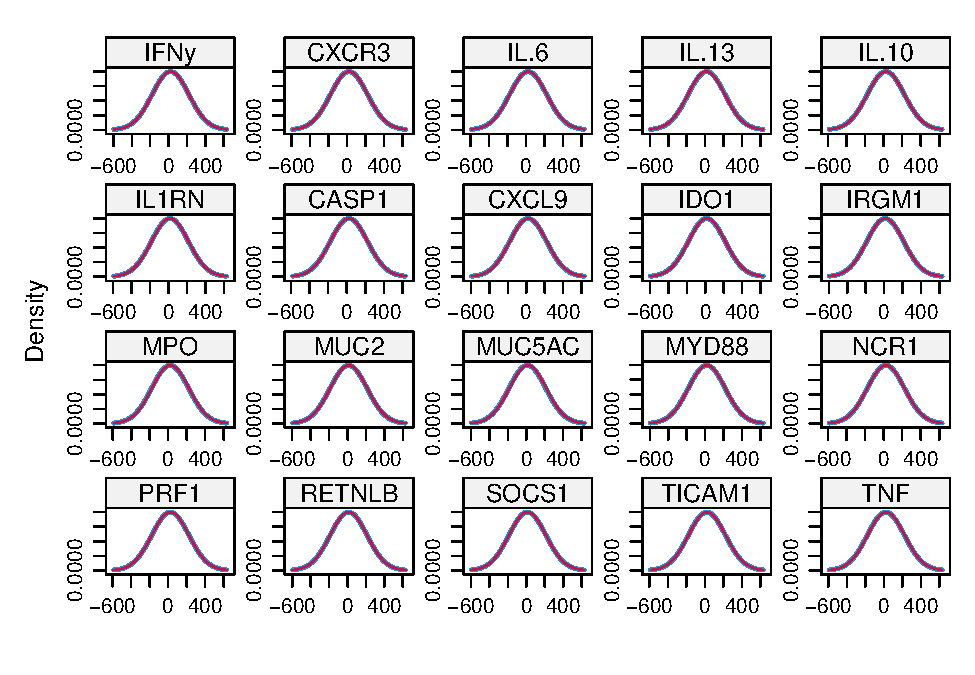
\includegraphics[width=1\linewidth]{Article_hybrids_tolerance_files/figure-latex/fig2-1} \caption{Density plot of observed and imputed data}\label{fig:fig2}
\end{figure*}

\hypertarget{results}{%
\section{Results}\label{results}}

\hypertarget{discussion}{%
\section{Discussion}\label{discussion}}

\hypertarget{conclusion}{%
\section{Conclusion}\label{conclusion}}

\hypertarget{a-subsection}{%
\subsection{A subsection}\label{a-subsection}}

\hypertarget{literature-citations}{%
\section{Literature citations}\label{literature-citations}}

\hypertarget{equations}{%
\section{Equations}\label{equations}}

An equation without a label for cross-referencing:

\[
E=mc^2
\]

An inline equation: \(y=ax+b\)

An equation with a label for cross-referencing:

\begin{equation}\label{eq:eq1}
\int^{r_2}_0 F(r,\varphi){\rm d}r\,{\rm d}\varphi = 1
\end{equation}

This equation can be referenced as follows: Eq. \ref{eq:eq1}

\hypertarget{inserting-r-figures}{%
\section{Inserting R figures}\label{inserting-r-figures}}

The code below creates a figure. The code is included in the output
because \texttt{echo=TRUE}.

\begin{Shaded}
\begin{Highlighting}[]
\FunctionTok{plot}\NormalTok{(}\DecValTok{1}\SpecialCharTok{:}\DecValTok{10}\NormalTok{,}\AttributeTok{main=}\StringTok{"Some data"}\NormalTok{,}\AttributeTok{xlab=}\StringTok{"Distance (cm)"}\NormalTok{,}
     \AttributeTok{ylab=}\StringTok{"Time (hours)"}\NormalTok{)}
\end{Highlighting}
\end{Shaded}

\begin{figure}[th]
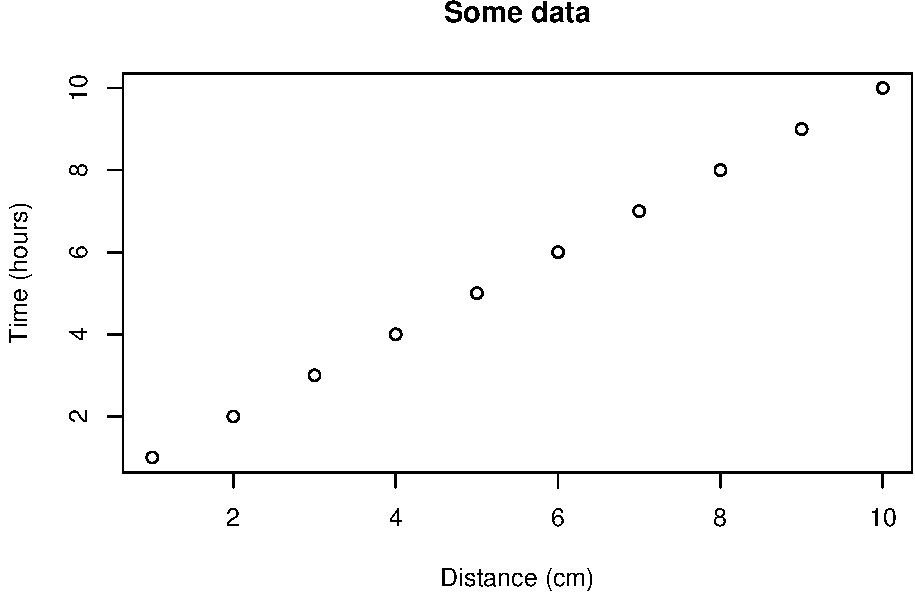
\includegraphics[width=1\linewidth]{Article_hybrids_tolerance_files/figure-latex/figa-1} \caption{This is the first figure.}\label{fig:figa}
\end{figure}

You can reference this figure as follows: Fig. \ref{fig:fig1}.

\hypertarget{figures-spanning-two-columns}{%
\subsection{Figures spanning
two-columns}\label{figures-spanning-two-columns}}

Figures can span two columns be setting \texttt{fig.env="figure*"}.

\begin{figure*}[th]
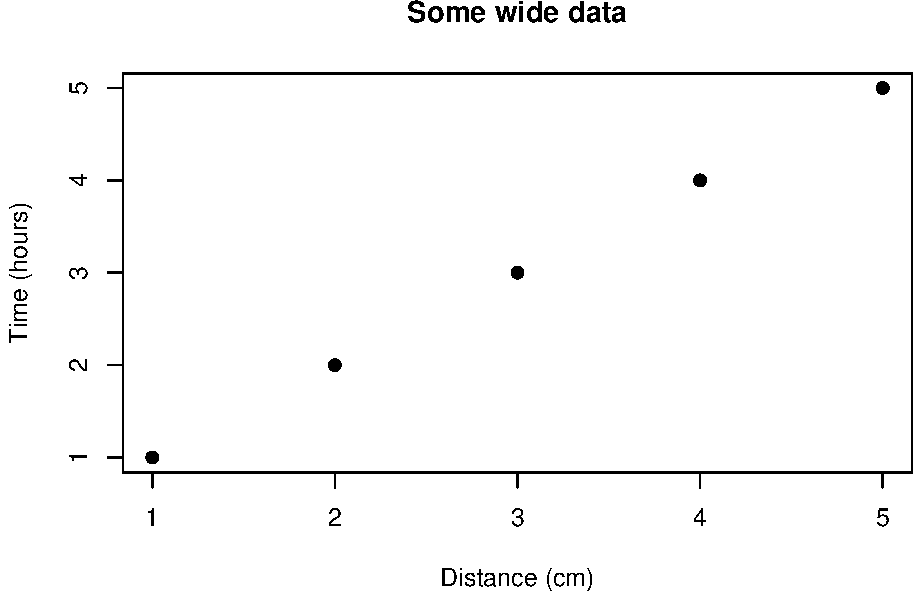
\includegraphics[width=1\linewidth]{Article_hybrids_tolerance_files/figure-latex/figb-1} \caption{This is a wide figure.}\label{fig:figb}
\end{figure*}

Reference to second figure: Fig. \ref{fig:fig2}

\hypertarget{tables}{%
\section{Tables}\label{tables}}

\hypertarget{generate-a-table-using-xtable}{%
\subsection{\texorpdfstring{Generate a table using
\texttt{xtable}}{Generate a table using xtable}}\label{generate-a-table-using-xtable}}

\begin{Shaded}
\begin{Highlighting}[]
\NormalTok{df }\OtherTok{=} \FunctionTok{data.frame}\NormalTok{(}\AttributeTok{ID=}\DecValTok{1}\SpecialCharTok{:}\DecValTok{3}\NormalTok{,}\AttributeTok{code=}\NormalTok{letters[}\DecValTok{1}\SpecialCharTok{:}\DecValTok{3}\NormalTok{])}

\CommentTok{\# Creates tables that follow OUP guidelines }
\CommentTok{\# using xtable}
\FunctionTok{library}\NormalTok{(xtable) }
\end{Highlighting}
\end{Shaded}

\begin{verbatim}
## Warning: package 'xtable' was built under R version 4.2.1
\end{verbatim}

\begin{Shaded}
\begin{Highlighting}[]
\FunctionTok{print}\NormalTok{(}\FunctionTok{xtable}\NormalTok{(df,}\AttributeTok{caption=}\StringTok{"This is a xtable table."}\NormalTok{,}
             \AttributeTok{label=}\StringTok{"tab:tab1"}\NormalTok{),}
      \AttributeTok{comment=}\ConstantTok{FALSE}\NormalTok{,}\AttributeTok{caption.placement=}\StringTok{"top"}\NormalTok{)}
\end{Highlighting}
\end{Shaded}

\begin{table}[ht]
\centering
\caption{This is a xtable table.} 
\label{tab:tab1}
\begin{tabular}{rrl}
  \hline
 & ID & code \\ 
  \hline
1 &   1 & a \\ 
  2 &   2 & b \\ 
  3 &   3 & c \\ 
   \hline
\end{tabular}
\end{table}

You can reference this table as follows: Table \ref{tab:tab1}.

\hypertarget{generate-a-table-using-kable}{%
\subsection{\texorpdfstring{Generate a table using
\texttt{kable}}{Generate a table using kable}}\label{generate-a-table-using-kable}}

\begin{Shaded}
\begin{Highlighting}[]
\NormalTok{df }\OtherTok{=} \FunctionTok{data.frame}\NormalTok{(}\AttributeTok{ID=}\DecValTok{1}\SpecialCharTok{:}\DecValTok{3}\NormalTok{,}\AttributeTok{code=}\NormalTok{letters[}\DecValTok{1}\SpecialCharTok{:}\DecValTok{3}\NormalTok{])}

\CommentTok{\# kable can alse be used for creating tables}
\NormalTok{knitr}\SpecialCharTok{::}\FunctionTok{kable}\NormalTok{(df,}\AttributeTok{caption=}\StringTok{"This is a kable table."}\NormalTok{,}
             \AttributeTok{booktabs=}\ConstantTok{TRUE}\NormalTok{,}\AttributeTok{label=}\StringTok{"tab2"}\NormalTok{)}
\end{Highlighting}
\end{Shaded}

\begin{table}

\caption{\label{tab:tab2}This is a kable table.}
\centering
\begin{tabular}[t]{rl}
\toprule
ID & code\\
\midrule
1 & a\\
2 & b\\
3 & c\\
\bottomrule
\end{tabular}
\end{table}

You can reference this table as follows: Table \ref{tab:tab2}.

\hypertarget{table-spanning-two-columns}{%
\subsection{Table spanning two
columns}\label{table-spanning-two-columns}}

Tables can span two columns be setting \texttt{table.envir\ =\ "table*"}
in \texttt{knitr::kable}.

\begin{Shaded}
\begin{Highlighting}[]
\NormalTok{df }\OtherTok{=} \FunctionTok{data.frame}\NormalTok{(}\AttributeTok{ID=}\DecValTok{1}\SpecialCharTok{:}\DecValTok{3}\NormalTok{,}\AttributeTok{code1=}\NormalTok{letters[}\DecValTok{1}\SpecialCharTok{:}\DecValTok{3}\NormalTok{],}
                \AttributeTok{code2=}\NormalTok{letters[}\DecValTok{4}\SpecialCharTok{:}\DecValTok{6}\NormalTok{],}
                \AttributeTok{code3=}\NormalTok{letters[}\DecValTok{7}\SpecialCharTok{:}\DecValTok{9}\NormalTok{],}
                \AttributeTok{code4=}\NormalTok{letters[}\DecValTok{10}\SpecialCharTok{:}\DecValTok{12}\NormalTok{],}
                \AttributeTok{code5=}\NormalTok{letters[}\DecValTok{13}\SpecialCharTok{:}\DecValTok{15}\NormalTok{])}

\CommentTok{\# kable can alse be used for creating tables}
\NormalTok{knitr}\SpecialCharTok{::}\FunctionTok{kable}\NormalTok{(df,}\AttributeTok{caption=}\StringTok{"This is a wide kable table."}\NormalTok{,}
             \CommentTok{\#format="latex",}
             \AttributeTok{table.envir=}\StringTok{"table*"}\NormalTok{,}
             \AttributeTok{booktabs=}\ConstantTok{TRUE}\NormalTok{,}\AttributeTok{label=}\StringTok{"tab3"}\NormalTok{)}
\end{Highlighting}
\end{Shaded}

\begin{table*}

\caption{\label{tab:tab3}This is a wide kable table.}
\centering
\begin{tabular}[t]{rlllll}
\toprule
ID & code1 & code2 & code3 & code4 & code5\\
\midrule
1 & a & d & g & j & m\\
2 & b & e & h & k & n\\
3 & c & f & i & l & o\\
\bottomrule
\end{tabular}
\end{table*}

\hypertarget{cross-referencing-sections}{%
\section{Cross-referencing sections}\label{cross-referencing-sections}}

You can cross-reference sections and subsections as follows: Section
\ref{literature-citations} and Section \ref{a-subsection}.

\textbf{\emph{Note:}} the last section in the document will be used as
the section title for the bibliography.

For more portable and flexible referencing of sections, equations,
figures and tables, use
\href{https://github.com/rstudio/bookdown}{\texttt{bookdown::pdf\_document2}}
with YAML header option \texttt{base\_format:\ rticles::oup\_article}.

\hypertarget{appendices}{%
\section*{Appendices}\label{appendices}}
\addcontentsline{toc}{section}{Appendices}

\begin{appendices}

\hypertarget{section-title-of-first-appendix}{%
\section{Section title of first
appendix}\label{section-title-of-first-appendix}}

blabla

\hypertarget{subsection-title-of-first-appendix}{%
\subsection{Subsection title of first
appendix}\label{subsection-title-of-first-appendix}}

and so on\ldots.

\end{appendices}

\section{Competing interests}

There are no competing interest.

\section{Author contributions statement}

To be worked on


\renewcommand\refname{References}

\bibliographystyle{abbrvnat}
\bibliography{mybibfile.bib}

%% Author bio-pics with images


\end{document}
